\documentclass[runningheads]{llncs}
\usepackage{times}
\usepackage{amsmath}
\usepackage{amssymb}
\usepackage{algorithm}
\usepackage[noend]{algpseudocode}
%\usepackage[noend]{algcompatible}
%\usepackage[ruled,linesnumbered,noend,oldcommands]{algorithm2e}
\usepackage[T1]{fontenc}
\usepackage{hyperref}
\usepackage{xspace}
\usepackage{graphicx}
\usepackage{listings}
\usepackage[table]{xcolor}
\usepackage{theorem}

\algrenewcommand\algorithmicprocedure{}
\algrenewcommand\algorithmicthen{}
\algrenewcommand\algorithmicdo{}
\definecolor{linen}{rgb}{0.98, 0.94, 0.9}
\definecolor{lightcyan}{rgb}{0.88, 1.0, 1.0}

\lstset { %
  language=C++,
  % backgroundcolor=\color{black!5}, % set backgroundcolor
  basicstyle=\footnotesize,% basic font setting
}

\renewcommand{\note}[1]{{\color{red}{#1}}}
\newcommand{\fs}[1]{\fontsize{#1}{#1}\selectfont}
\newcommand{\fss}[2]{\fontsize{#1}{#2}\selectfont}
\newcommand{\sat}{SAT\xspace}
\newcommand{\trail}{\ensuremath{\mathcal{T}}}
\newcommand{\trailIdxT}[2]{\ensuremath{\iota_{#1}(#2)}}
\newcommand{\trailIdx}[1]{\ensuremath{\iota(#1)}}
\newcommand{\range}[2]{#1\ldots#2}
\newcommand{\dlevel}[1]{\ensuremath{\mathit{decLvl}(#1)}}
\newcommand{\dlevels}{\ensuremath{\mathit{decLvls}}}
\newcommand{\var}{\text{var}}
\newcommand{\true}{\textsc{true}\xspace}
\newcommand{\false}{\textsc{false}\xspace}
\newcommand{\reason}[1]{\ensuremath{\mathit{reason}(#1)}}
\newcommand{\reasonsave}[1]{\ensuremath{\mathit{reason_{\mathit{save}}(#1)}}}
\newcommand{\litsave}{\ensuremath{\mathit{l_{\mathit{save}}}}}
\newcommand{\formula}{\ensuremath{\mathcal{F}}}
\renewcommand{\implies}{\rightarrow}
\newcommand{\uipcls}{C_{\textit{1-UIP}}}
\newcommand{\deepestLvl}{L_{\textit{deep}}}
\newcommand{\deepestLit}{\ell_{\textit{deep}}}
\newcommand{\btL}{L_{\textit{back}}}
\newcommand{\cbt}{C-bt\xspace}
\newcommand{\trailsave}{\trail_{\mathit{save}}}
\newcommand{\bt}{\textsc{backtrack}\xspace}
\newcommand{\ust}{\textsc{useSavedTrail}\xspace}

\newtheorem{Obs}{Observation}
\newtheorem{Cor}{Corollary}
\newtheorem{defn}{Definition}
\newtheorem{thm}{Theorem}
\newtheorem{prop}{Proposition}
\newtheorem{ex}{Example}
\newcommand{\whitebox}{\raisebox{.5ex}{\fbox{\hspace*{.2ex}}}}

\title{Trail Saving on Backtrack}
\author{Randy Hickey \and Fahiem Bacchus}
\institute{Department of Computer Science, University of Toronto, Canada\\
  \email{rgh000@gmail.com, fbacchus@cs.toronto.edu}}

\begin{document}
\maketitle
\begin{abstract}
    A CDCL \sat solver can backtrack a large distance when it learns a
    new clause, e.g, when the new learnt clause is a unit clause the
    solver has to backtrack to level zero. When the length of the
    backtrack is large, the solver can end up reproducing many of the
    same decisions and propagations when it redescends the search
    tree. Motivated by this potential redundancy, partial backtracking
    (chronological backtracking) has been proposed. This technique
    allows the solver to reduce the length of its backtrack, e.g.,
    allowing the solver to backtrack to the previous level after a
    conflict is found. However, this technique has its shortcomings
    and only tends to work when limits are placed on its
    application. In this paper we present a new trail saving technique
    that makes a copy of the part of the trail that was backtracked
    over. This saved copy can then be used to improve the efficiency
    of the solver's subsequent redescent. Although our technique does
    not save as much work as chronological backtracking, it also does
    not have chronological backtracking's shortcomings. Furthermore,
    the saved trail also provides the solver with the ability to look
    ahead along the previous trail. This can be exploited to improve
    its efficiency. Our empirical results show that our technique
    often yields superior performance over chronological backtracking,
    and that is is able to improve the performance of state-of-the-art
    solvers.

\end{abstract}

\section{Introduction}
\textbf{Overall message of the paper.}

% \begin{enumerate}
% \item Formalism for understanding a more general form of trail savings
%     which caches a copy of the trail that is backtracked over, and
%     verifying how it exploited soundly.

% \item Potential advantages over chronological backtracking.  Literals
%     remain at the correct level, supports the solver having more
%     freedom in its decisions.

% \item Potential advantages of technique (1) increase in efficiency of
%     propagation, (2) the new uses of the cached information. 

% \item Potential disadvantage. Reasons are recycled, in some circumstances
%     new reasons might be better. We show in a simple experiment that
%     this effect can occur.

% \item Technique captures most of the positive effects of
%     non-chronological backtracking in a simpler to implement way. It
%     also preserves the simpler standard structure of CDCL
%     solvers. Already provides some advantages for current SAT
%     solvers. The ideas also have the potential for further
%     exploitation. Lookahead for conflicts seems to be beneficial, and
%     potentially if better discrimatory measures could be developed for
%     reason clauses we could also better determine whether or not to
%     use the cached information.. 
% \end{enumerate}

% \note{Reusing the Assignment Trail in CDCL Solvers: restart to level
%   $i$ where the next decision has a higher score than the decision at
%   level $i$ and a lower score than all decisions at level $j$ for
%   $j< i$.

%   They argum changes to reason clauses don't make much difference, but
%   that was with minisat, before metrics for clause quality were in place in sat solvers.

%   The savings for Luby-100 (used in minisat) were about 1\%}

The vast majority of modern SAT solvers that are used to solve
real-world problems are based on the conflict-driven clause learning
(CDCL) algorithm. In a CDCL SAT solver, backtracking occurs after
every conflict, where all literals from one or more decision levels
become unassigned, before the solver resumes making decisions and
performing unit propagations. Traditionally, CDCL solvers would
backtrack non-chronologically to the conflict level, which is the
second highest decision level remaining in the conflict clause after
conflict analysis has resolved away all but one literal from the
current decision level \cite{DBLP:conf/dac/MoskewiczMZZM01}. Recently,
however, it has been shown that partial backtracking
\cite{DBLP:conf/lpar/JiangZ13} or chronological backtracking, \cbt,
(i.e. backtracking one level only after conflict analysis)
\cite{DBLP:conf/sat/NadelR18,DBLP:conf/sat/MohleB19} can be effective
on many instances and was implemented in solvers that won the last two
SAT competitions. Although chronological backtracking breaks some of
the conventional invariants of CDCL solvers, it has been formalized
and proven correct \cite{DBLP:conf/sat/MohleB19}.

The motivation for using \cbt is the observation that when a solver
backtracks across many levels, many of the literals that are
unassigned during the backtrack will be re-assigned again in roughly
the same order when the solver redescends. This observation was first
made in the context of restarts by van der Tak et
al. \cite{DBLP:journals/jsat/TakRH11}. Their technique backtracks to
the minimum change level, i.e., the first level at which the solver's
trail can change on redescent. However, their technique cannot be used
when backtracking from a conflict: the solver's trail is going to be
changed at the backtrack level so the minimum change level is the same
as the backtrack level. 

Chronological backtracking or partial backtracking instead allows a
reduction in the length of the backtrack by placing literals on the
trail out of decision level order. By reducing the length of the
backtrack the solver can keep more of its assignment trail
intact. This can save it from the work involved in reconstructing a
lot of its trail. Using \cbt is not a panacea however. Its application
must be limited for peak effectiveness. This indicates that it is
sometimes beneficial for the solver to backtrack fully and redo its
trail, even if this takes more work. We will expand on why this might
be the case below.

In this paper we present an alternative ``trail saving'' method whereby
we save the backtracked part of the solver's trail and attempt to
use that information to make the solver's redescent more
efficient. Trail saving preserves the traditional invariants of the
SAT solver and its basic version is very simple to implement. It
allows the search to retain complete control over the order of
decisions, but helps make propagation faster. We develop some
enhancements to make the idea more effective, and demonstrate
experimentally that it performs as well as and sometimes better than
chronological backtracking. We also show that with the enhancements we
are able to improve the performance of state-of-the-art solvers. 

\section{Background}
\label{sec:background}
\sat solvers determine the satisfiability of a propositional formula
$\formula$ expressed in Conjunctive Normal Form (CNF). $\formula$
contains a set of variables $V$. A literal is a variable $v\in V$ or
its negation $\lnot v$, and for a literal $l$ we let $\var(l)$ denote
its underlying variable. A CNF consists of a conjunction of clauses,
each of which is a disjunction of literals. We often view a clause as
being a set of literals and employ set notation, e.g., $\ell\in C$ and
$C'\subset C$. We will assume that the reader is familiar with the
basic operations of CDCL \sat solvers. A good source for this
background is \cite{DBLP:series/faia/SilvaLM09}.

\paragraph{Trails.}
CDCL \sat solvers maintain a trail which is the sequence of literals
that have currently been assigned \true by the solver. During its
operation a \sat solver will add newly assigned literals to the end of
the trail, and on backtrack remove literals from the end of the
trail. For convenience, we will regard \emph{literals as having been
  assigned \true if and only if they are on the trail}. So
removing/adding a literal to the trail is equivalent to
unassigning/assigning the literal $\true$.

A \sat solver's trail satisfies a number of conditions. However, in
this work we will need some additional flexibility in our definitions,
as we will sometimes be working with trails that would never be
constructed by a \sat solver. Hence, we define a \emph{trail} to be a
sequence of literals each of which is either a \emph{decision} literal
or an \emph{implied} literal, and each of which has a
\emph{reason}. These two types of literals are distinguished by their
\emph{reasons}. Decision literals $d$ have a null reason,
$\reason{d} = \varnothing$. Implied literals $l$ have as a reason a
clause of the formula $\formula$, $\reason{l} =
C\in\formula$. (The clause $\reason{l}$ can be a learnt clause that has been
added to $\formula$).

If literal $\ell$ is on the trail $\trail$ let
$\trailIdxT{\trail}{\ell}$ denote its index on the trail, i.e,
$\trail[\trailIdxT{\trail}{\ell}] = \ell$. If $x$ and $y$ are both on
the trail and $\trailIdxT{\trail}{x} < \trailIdxT{\trail}{y}$ we say
that \textit{$x$ appears before $y$ on the trail}. For convenience,
when the trail being discussed is clear from context we simply write
$\iota$ instead of $\iota_{\trail}$.

Each literal $\ell\in\trail$ has a decision level $\dlevel{\ell}$
which is equal to the number of decision literals appearing on the trail
up to and including $\ell$; hence, $\dlevel{d}=1$ for the first
decision literal $d\in\trail$. The set of literals on $\trail$ that
have the same decision level forms a \emph{contiguous}
subsequence\footnote{Our approach uses standard trails in which the
  decision levels are contiguous. Chronological backtracking
  \cite{DBLP:conf/lpar/JiangZ13,DBLP:conf/sat/NadelR18,DBLP:conf/sat/MohleB19}
  generates trails with non-contiguous decision levels} that starts
with a decision literal $d_i$ and ends just before the next decision
literal $d_{i+1}$. We will often need to refer to different decision
level subsequences of $\trail$. Hence, we let $\trail[[i]]$ denote the
subsequence of literals at decision level $i$; and let
$\trail[[\range{i}{j}]]$ denote the subsequence of literals at
decision levels $k$ for $i\leq k\leq j$. 
\begin{defn}
    A clause $C$ has \textbf{been made unit by $\trail$ implying $l$}
    when
    $l\in C \land \bigl(\forall x\in C. x\neq l \implies \lnot x \in
    \trail\bigr)$. That is, all literals in $C$ except $l$ must have
    been falsified by $\trail$
\end{defn}

Now we define the following properties that a trail $\trail$ can have.
\begin{description}
\item[non-contradictory:] A variable cannot appear in both polarities
    in the trail: $l\in \trail\implies \lnot l \not \in \trail$.
\item[non-redundant:] A literal can only appear once on $\trail$.
\item[reason-sound:] For each implied literal $l\in\trail$ we have
    that its reason clause $\reason{l}=C$ has been made unit by
    $\trail$ implying $l$, and for each $x\in C$ with $x\neq l$ we
    have that $\lnot x$ appears before $l$ on $\trail$:
    $\forall l\in\trail.\, \reason{l}\neq \varnothing \implies
    l\in\reason{l} \land \bigl(\forall x\in\reason{l}.\, x\neq l
    \implies \lnot x \in \trail \land \trailIdx{\lnot x} <
    \trailIdx{l}\bigr)$.
\item[propagation-complete:] Unit propagation has been run to
    completion at all decisions levels of $\trail$. This means that
    literals appear on $\trail$ at the first decision level they were
    unit implied. Formally, this can be captured by the condition:
    $\forall i \in \{\dlevel{l}\,|\,l\in \trail\}. \bigl(\exists
    C\in\formula. \mbox{$C$ is made unit by $\trail[[\range{0}{i}]]$
      implying $l$}\bigr) \implies l\in \trail[[\range{0}{i}]]$. Note
    that propagation completeness implies that
    $\reason{l}\neq \varnothing$ must contain at least one other
    literal $y\neq l$ with $\dlevel{y} = \dlevel{l}$.
\item[conflict-free:] No clause of $F$ is falsified by
    $\trail$. Clauses $C\in F$ falsified by $\trail$ are typically
    called \emph{conflicts}.
\end{description}

In CDCL solvers using standard conflict directed backtracking all
properties hold of the prefix of the solver's trail consisting of all
decisions levels but the deepest. The full trail might, however,
contain a conflict at its deepest level so is not necessarily conflict-
free. The full trail might also not be propagation-complete, as unit
propagation at the deepest level is typically terminated early if a
conflict is found. It can further be noted that the first four
properties imply that if a clause $C$ is falsified at decision level
$k$, then $C$ must contain at least two literals at level $k$
(otherwise $C$ would have become unit at a prior level and then
satisfied by making its last unfalsified literal \true).

\paragraph{Standard Backtracking.}
In CDCL \sat solving the solver extends its trail by adding new
decision literals followed by finding and adding all unit implied
literals arising from that new decision. This continues until it
reaches a decision level $\deepestLvl$ where a conflict $C$ is found.

In standard backtracking, the solver then constructs a new 1-UIP
clause by resolving away all but one literal at level $\deepestLvl$
from the conflict $C$ using the reason clauses of these literals. (As
noted above $C$ must contain at least two literals at level
$\deepestLvl$). Hence, the new clause $\uipcls$ will contain one
literal $\deepestLit$ at level $\deepestLvl$ and have all of its other
literals a levels less than $\deepestLvl$. The solver then backtracks
to $\btL$ the second deepest level in $\uipcls$. This involves
changing $\trail$ to its prefix $\trail[[\range{0}{\btL}]]$ (by our
convention all literals removed from $\trail$ are now unassigned). The
new clause $\uipcls$ is made unit by $\trail[[\range{0}{\btL}]]$
implying $\deepestLit$, so the solver then adds $\deepestLit$ to the
trail and executes another round of unit propagation at level $\btL$,
after which it continues by once again growing the trail with new
decisions and unit implied literals until a new conflict or a
satisfying assignment is found.

In standard backtracking, the difference between the backtrack level,
$\btL$ and the current deepest level $\deepestLvl$ can be very
large. During its new descent from $\btL$ the solver can reproduce a
large number of the same decisions and unit propagations, essentially
wasting work. This potential inefficiency has been noted in prior work
\cite{DBLP:journals/jsat/TakRH11,DBLP:conf/lpar/JiangZ13,DBLP:conf/sat/NadelR18,DBLP:conf/sat/MohleB19}.

In \cite{DBLP:journals/jsat/TakRH11} a technique for reducing the
length of the backtrack during restarts was presented. In restarts,
the solver backtracks to level $0$, and this technique involves
computing a new deeper backtrack level $M> 0$ for which it is known
that on redescent the first $M+1$ levels of the trail will be
unchanged (except perhaps for the ordering of the literals). This
technique removes the redundant work of reproducing the first $M$
trail levels. When backtracking from a conflict, however, the trail
will be changed at level $\btL$ ($\deepestLit$ will be newly inserted
at this level). Hence this technique cannot reduce the length of the
backtrack. In this paper we will show that although we have to
backtrack to $\btL$ we can make the subsequent redescent much more
efficient.

\paragraph{Chronological Backtracking.}
Chronological bactracking (\cbt) is a technique originally proposed by
Jiang and Zhang \cite{DBLP:conf/lpar/JiangZ13} under the name
\textit{partial backtracking}. Its aim is to reduce the redundant work
that might be done by the \sat solver on its redescent from the
backtrack level $\btL$. The original paper proposed a technique for
backtracking to any level $j$ in the range
$\btL \leq j \leq \deepestLvl{-}1$ (where $\deepestLvl$ is the level
the conflict was discovered). Nadel and Ryvchin
\cite{DBLP:conf/sat/NadelR18} proposed to always backtrack to
$\deepestLvl{-}1$ while M{\"{o}}hle and Biere
\cite{DBLP:conf/sat/MohleB19} returned to the original proposal of
flexibly backtracking to any level in the allowed range. Note that the
new 1-UIP clause $\uipcls$ is made unit at every level in this
range. So after backtracking to level $j$ the newly implied literal
$\deepestLit$ can be added to the trail with
$\reason{\deepestLit}=\uipcls$, and $\dlevel{\deepestLit}$ is set to
$\btL$ (the second deepest level in $\uipcls$.

This means that the decision levels on the trail are no longer
contiguous, as $\deepestLit$ has a different level than the other
literals at level $j$ (if $j\neq \btL$). This change has a number of
consequences for the \sat solver's operation, all of which were
described in the original paper \cite{DBLP:conf/lpar/JiangZ13}. In
\cite{DBLP:conf/sat/NadelR18} some more practical implementation
methods were developed to overcome this issues, and in
\cite{DBLP:conf/sat/MohleB19} a formal framework for \cbt was
developed under which the changes required to the \sat solver could be
shown to be sound. We refer the reader to the cited papers for
more details.

\section{Potential Drawbacks of Chronological Backtracking}
In this paper we present a new technique that allows the \sat solver
to use standard backtracking, but also allows saving some redundant
work on its redescent.  Our method has more overhead than \cbt so the
first question that must be addressed is why not just use
chronological backtracking.

The reduction in redundant work achieved by \cbt does not come for
free. In particular, some of the work avoided by \cbt is not actually
redundant work; it is work that can actually help the solver. The
obvious evidence for this statement is that in both
\cite{DBLP:conf/sat/NadelR18} and \cite{DBLP:conf/sat/MohleB19} it was
found that it was not optimal to always apply \cbt. In
\cite{DBLP:conf/sat/NadelR18} \cbt was applied only when the length of
the standard backtrack, $\btL-\deepestLvl$ was greater than a given
threshold $T$. In their experiments they found that $T=100$ was the
best value, i.e., \cbt is done only on longer backtracks. In practice,
this meant that \cbt was \emph{hardly ever done}; in our measurements
with their solver only about 3\% of the solver backtracks were \cbt
backtracks. In \cite{DBLP:conf/sat/MohleB19} the value $T=100$ was
also applied. However, they introduced an additional technique to add
some applications of \cbt when the length of the backtrack is less
than $T$. This allowed \cite{DBLP:conf/sat/MohleB19} to utilize \cbt
in about \%15 of the backtracks. Nevertheless, the fact \cbt has to be used
in a controlled fashion, indicates that there can be benefits in the \sat
solver employing standard backtracking; it cannot be the case that
every redescent is only doing redundant work.

What is this non-redundant work? With standard backtracking the
literal $\deepestLit$ is placed on the trail at the end of $\btL$ and
then unit propagated. This could impact the trail in at least the
following ways. First, some literals might become unit at earlier
levels. This could include decision literals becoming forced which
might compress some decision levels together. Second, different
decisions might be made due to changes in the variable scores arising
from the newly learnt clause. And third, literals might be unit
implied with different reasons. These changes could have a major
impact on the future learnt clauses, and thus on the solver's
efficiency. Unfortunately, it seems difficult to predict when these
impacts might be large.

The second impact, changing variable scores, is partially addressed in
\cite{DBLP:conf/sat/MohleB19} who utilize the ideas of
\cite{DBLP:journals/jsat/TakRH11} to backtrack to a level where the
decisions would be unchanged. However, if the length of the backtrack
is greater than $100$ there could still be a divergence between the
variable decisions generated by standard backtracking and \cbt. An
argument is also given in \cite{DBLP:journals/jsat/TakRH11} that the
third impact, changing literal reasons, is not significant. However,
the experiments in \cite{DBLP:journals/jsat/TakRH11} were run before
good notions of clause quality were known
\cite{DBLP:conf/ijcai/AudemardS09}. Our empirical results indicate
that once clause quality is accounted for changing the literal reasons
can have a significant impact.

The first impact is worth discussing since it was mentioned in the
original \cbt paper \cite{DBLP:conf/lpar/JiangZ13} but not in the
subsequent works. This is the issue of changing the decision levels of
literals on the trail. \cbt computes the decision level of each
implied literal based on the decision levels of its reasons, but it
does not go backwards to change the decisions levels of literals
earlier on the trail.

\begin{example}
    For example, suppose that $(x, \lnot y)\in \formula$, the literal $x$
    is a decision literal on the trail with $\dlevel{x}=2$, and that
    the solver is currently at level $150$ where it encounters a
    conflict. If this conflict yields the unit clause $(y)$, standard
    backtracking would backtrack to level $0$, where $x$ would be
    implied. On redescent, $x$ would no longer form a new decision
    level and it would not appear in any new clauses (as it is
    entailed by $\formula$). \cbt, on the other hand, would backtrack
    to level $149$. On its trail $x$ would still be at level
    $2$. Until a backtrack past level $2$ occurs, learnt clauses might
    contain $\lnot x$, and thus have level $2$ added to their set of
    levels (potentially changing their LBD score). Only when backtrack
    past level $2$ occurs would $x$ be restored to its correct level
    $0$, and it would require inprocessing simplifications to remove $x$
    from the learnt clauses.
\end{example}

In sum, although these impacts of \cbt might or might not be harmful
to the \sat solver, they exist. Hence, perhaps the most unappealing
aspect of \cbt is that it introduces additional interdependencies
between components of the solver. For example, the second impact means
that heuristics for choosing decision variables might work differently
in the presence of \cbt; and the first impact means that different
ways of computing clause quality using the decision levels in the
clauses might also work differently in the presence of \cbt. So
although there are bound to be cases where \cbt is superior, we would
like to have a method that addresses the original motivation of
reducing redundant work while not changing the operation of standard
backtracking. We present our proposal for such a method next.

\section{Trail Saving}
Our approach is to save the trail $\trail$ on backtrack, and to use
the saved trail $\trailsave$ when the solver redescends to improve the
efficiency of propagations without affecting the decisions the solver
wants to make. The saved trail $\trailsave$ also provides a secondary
``lookahead mechanism'' that the \sat solver can exploit as it
redescends.

Suppose that the solver is at $\deepestLvl$ where it has encountered a
conflict. From the 1-UIP clause it learns, $\uipcls$, it now has to
backtrack to $\btL$. This is accomplished by calling
\textsc{backtrack($\btL$)}, shown in Figure~\ref{fig:trailUse}, which
saves the backtracked portion of the trail.

Note that \bt does not save the deepest level of $\trail$. The full
$\trail$ contains a conflict (at its deepest level). Hence the solver
will never reproduce all the same levels, and it would be useless to
save all of them. Note also that in addition to saving the literals in
$\trailsave$ we also save the clause reason of the unit implied
literals in a separate $\mathit{reason_{save}}$ vector. Finally, we
see that after backtrack the first literal on $\trailsave$ is a
decision literal: it is the first literal of $\trail$ at decision
level $\btL+1$. Literals will be removed from $\trailsave$ during its
use, but always in units of complete decision levels. So
$\trailsave[0]$ will always be a (previous) decision literal.

After backtrack the solver will add $\deepestLit$ to the end of the
updated $\trail$ with $\reason{\deepestLit}$ $\mbox{}=\uipcls$ and
then invoke unit propagation. $\trailsave$ is exploited during
propagation by the version of \textsc{propagate} shown in
Figure~\ref{fig:trailUse}, which will initially be invoked with the
argument $\trailIdx{\deepestLit}$ (i.e., the trail index of the newly
added implicant). The saved trail will be continually consulted during the
solver's descent whenever unit propagation is performed. When
backtrack occurs $\trailsave$ will be overwritten to store the new
backtracked portion of $\trail$.

\begin{figure}[!t]
\begin{algorithmic}[1]
    \Procedure{backtrack}{$\btL$}
    \State $\forall \ell\in\trail[[\range{\btL{+}1}{\deepestLvl{-}1}]]$ $\reasonsave{\ell} = \reason{\ell}$
    \State $\trailsave = \trail[[\range{\btL{+}1}{\deepestLvl{-}1}]]$\label{ln:btsave}
    \State $\trail = \trail[[\range{0}{\btL}]]$
    \EndProcedure
\end{algorithmic}

\begin{algorithmic}[1]
    \Procedure{propagate}{idx}
    \While{idx $\mbox{} < \trail.\mathrm{size}$()}
        \State $c\gets\mbox{}$ \ust()
        \If{($c\neq \varnothing$)} \textbf{return} $c$ \Comment{Found conflict from $\trailsave$}
        \EndIf
        \State $\ell \gets \trail[idx]$
        \For{each clause $c\in$ watchlist($\lnot \ell$)}
            \If{($c$ is unit implying $x$)}
                 \State $\trail.\mathrm{addToEnd}(x)$; \; $\reason{x} \gets c$            
            \ElsIf{($c$ is falsified)}\:
                 \textbf{return} $c$ \Comment{Found conflict from unit prop.}
            \Else\:
                 Update $c$'s watches.
            \EndIf
        \EndFor
        \State $idx$++
    \EndWhile
    \EndProcedure
    \Statex
    \Procedure{useSavedTrail}{\mbox{}}
    \State $idx\gets 0$; $c\gets \varnothing$
    \For{( ; $idx < \trailsave.\mathrm{size}()$; $idx$++)}
        \State $\litsave\gets \trailsave[idx]$
        \If{($\reasonsave{\litsave} = \varnothing$)} \Comment{Decision on $\trailsave$}
            \If{($\litsave\in\trail$)}\: \textbf{continue} \Comment{\true in solver, we can use its implied lits}
            \Else{}\: \textbf{break} \Comment{Only solver can set decisions, so we stop here}\label{ln:decnottrue}
            \EndIf
        \Else{} \Comment{Implied Literal on $\trailsave$}
             \If{($\litsave \in \trail$)}\: \textbf{continue}  \Comment{ignore redundant lits}\label{ln:skip}
             \ElsIf{($\lnot \litsave \in \trail$)} 
                \Comment{contradiction, return conflict and reset $idx$}\label{ln:conflict}
                 \State $c\gets\reasonsave{\litsave}$; $idx\gets 0$; \textbf{break}
             \Else{} \Comment{unset in solver, add to solver's trail}
                  \State $\trail.\mathrm{addToEnd(\litsave)}$\label{ln:addToTrail}
                  \State $\reason{\litsave}\gets \reasonsave{\litsave}$\label{ln:addToTrailNext}
              \EndIf
        \EndIf
    \EndFor
    \For{($i \gets 0$; $i < idx$; $i$++)} \Comment{$\trailsave$ is unchanged when $idx=0$}
        \State $\trailsave.\mathrm{removeFront()}$\label{ln:popfront}
    \EndFor
    \State \textbf{return} $c$
    \EndProcedure
\end{algorithmic}

\caption{Using $\trailsave$ in unit propagation and conflict
  detection} \label{fig:trailUse}
\end{figure}

$\trailsave$ is consulted in the procedure $\ust$
(Figure~\ref{fig:trailUse}). This procedure tries to add saved implied
literals and their reasons to the solver's trail, when these
implications are valid. We will show below that those implications
that are added are in fact valid. We do not interfere with the
solver's variable decisions. Instead we opportunistically test to see
if literals implied on $\trailsave$ are valid implications for the
solver given the solver's current decisions.

$\trailsave[0]$ is always a (previous) decision literal $d$ with
$\reasonsave{d}=\varnothing$. Note that, since new literals (e.g.,
$\deepestLit$) have been added to $\trail$, $d$ might now be an
implied literal on $\trail$ (i.e., $\reason{d}\neq\varnothing$) even
though before the backtrack it was previously a decision (i.e.,
$\reasonsave{d}=\varnothing$). If $d$ has not been assigned $\true$ by
the solver (i.e., $\lnot d \in \trail$), we cannot add any implied
literals below it on $\trailsave$ to $\trail$ as these implied
literals depend on $d$ being assigned $\true$. In this case we stop
looking for more literals to add to $\trail$
(line~\ref{ln:decnottrue}).

On the other hand if $d$ has been made \true by the solver we can
continue to add all of the implied literals below it (up to but not
including the next decision literal on $\trailsave$) to $\trail$
(line~\ref{ln:addToTrail}), reusing their saved reasons. Any literals
that have already been made true by the solver can be skipped
(line~\ref{ln:skip}). Finally, if we encounter a literal that has
already been falsified by the solver, then its saved reason clause
must be falsified by the solver and we can return it as a conflict
(line~\ref{ln:conflict}). If a conflict is encountered we leave
$\trailsave$ unchanged by resetting $idx$ to zero. Otherwise, $idx$
will be the number of literals at the front of $\trailsave$ that have
been moved to $\trail$ (or skipped over since they are already on
$\trail$). We then remove the first $idx$ literals from $\trailsave$
(line~\ref{ln:popfront}), and return the conflict (equal to
$\varnothing$ if no conflict was found).

\begin{figure}[!t]
\begin{tabular}{l
  >{\raggedleft}p{4.75ex}>{\raggedleft}p{4.75ex}>{\raggedleft}p{4.75ex}>{\raggedleft}p{4.75ex}
  >{\raggedleft}p{4.75ex}>{\raggedleft}p{4.75ex}>{\raggedleft}p{4.75ex}>{\raggedleft}p{4.75ex}
  >{\raggedleft}p{4.75ex}>{\raggedleft}p{4.75ex}>{\raggedleft}p{4.75ex}>{\raggedleft}p{4.75ex}
  >{\raggedleft}p{4.75ex}>{\raggedleft}p{4.75ex}}
      $\trail$ 
      & $l_1^{1*}$ & $l_2^1$ & $l_3^{2*}$ & $l_4^2$
      & $l_5^{3*}$ & $l_6^3$ & $l_7^{4*}$ & $l_8^4$
      & $l_9^{5*}$ & $l_{10}^5$ & $l_{11}^5$ & $l_{12}^{6*}$
      & $l_{13}^6$ & $l_{14}^6$  \tabularnewline
     $\trailsave$
      &  &  &  & 
      &  &  &  &  
      &  &  &  &  
      &  & \tabularnewline
      \rowcolor{linen}
      \multicolumn{15}{l}{1-UIP ($\lnot l_1$, $\lnot l_3$, $\lnot l_{12}$) and backtrack 2 ($\btL$)}\tabularnewline
      $\trail$ 
      & $l_1^{1*}$ & $l_2^1$ & $l_3^{2*}$ & $l_4^2$
      &         &       &         &      
      &         &       &         &           
      &         &         \tabularnewline
      $\trailsave$
      &         &       &         &                     
      & $l_5^*$ & $l_6$ & $l_7^*$ & $l_8$
      & $l_9^*$ & $l_{10}$ & $l_{11}$ & 
      &         & 
      \tabularnewline
      \rowcolor{linen}
      \multicolumn{15}{l}{Unit Prop $\lnot l_{12}$ ($\deepestLit$), $\trailsave$ not yet helpful}\tabularnewline
      $\trail$ 
      & $l_1^{1*}$ & $l_2^1$ & $l_3^{2*}$ & $l_4^2$
      & $\smash{\lnot} l_{12}^2$  & $l_7^2$  & $l_9^2$    &      
      &         &       &         &           
      &         &         \tabularnewline
      $\trailsave$
      &         &       &         &                     
      & $l_5^*$ & $l_6$ & $l_7^*$ & $l_8$
      & $l_9^*$ & $l_{10}$ & $l_{11}$ &
      &         & 
      \tabularnewline
      \rowcolor{linen}
      \multicolumn{15}{l}{Make decision}\tabularnewline
      $\trail$ 
      & $l_1^{1*}$ & $l_2^1$ & $l_3^{2*}$ & $l_4^2$
      & $\smash{\lnot} l_{12}^2$  & $l_7^2$  & $l_9^2$ 
      & $l_5^{3*}$  &       &         &           
      &         &         \tabularnewline
      $\trailsave$
      &         &       &         &                     
      & $l_5^*$ & $l_6$ & $l_7^*$ & $l_8$
      & $l_9^*$ & $l_{10}$ & $l_{11}$ & 
      &         & 
      \tabularnewline
      \rowcolor{linen}
      \multicolumn{15}{l}{Now $\trailsave$ can be used to augment trail}\tabularnewline
      $\trail$ 
      & $l_1^{1*}$ & $l_2^1$ & $l_3^{2*}$ & $l_4^2$
      & $\lnot l_{12}^2$ \hfill & $l_7^2$  & $l_9^2$      
      & $l_5^{3*}$  & $l_6^{3}$  & $l_8^3$  & $l_{10}^3$          
      & $l_{11}^3$  &         \tabularnewline
      $\trailsave$
      &         &       &         &      
      &         &       &                              
      &         &       &         & 
      &         &       & 
    \end{tabular}
    \caption{Use of $\trailsave$ from
      Example~\ref{ex:trailsave}\label{fig:trailsave}. The literal's
      decision level is indicated in its superscript, and a $\mbox{}^*$
      superscript indicates that the literal is a decision.}
\end{figure}

\begin{example}
    \label{ex:trailsave} Figure~\ref{fig:trailsave} provides an
    example of how $\trailsave$ is used. Initially the literals $l_1$
    to $l_{14}$ are on the solver's $\trail$, and $\trailsave$ is
    empty. This is shown in the first two lines of the figure. In the
    figure the superscript on the literals indicates their decision
    level, and a superscripted $*$ indicates that the literal is a
    decision. Hence $l_1^{1*}$ indicates that $\dlevel{l_1}=1$ and
    that $l_1$ is a decision.

    Then a conflict is found at level $6$ and the 1-UIP clause
    $(\lnot l_1, \lnot l_3, \lnot l_{12})$ is learnt. Thus the solver
    will backtrack to level $2$, where it will add $\lnot l_{12}$ as a
    unit implicant. The next two lines show $\trail$ and $\trailsave$
    right after the backtrack to level $2$: the backtracked levels
    have been copied into $\trailsave$ omitting the conflict level $6$. 

    The new unit $\lnot l_{12}$ is now added to $\trail$ and unit
    propagation performed adding $l_7$ and $l_9$ to level 2. Since the
    first literal on $\trailsave$, $l_5$, has
    $\reasonsave{l_5}=\varnothing$ ($l_5$ was a decision on $\trail$
    at the time backtrack occurred) and is not yet $\true$,
    $\trailsave$ is not helpful at this stage. The status of $\trail$
    and $\trailsave$ at this point is shown in the figure.
    
    After unit propagation is finished the solver makes a new
    decision, which happens to be (but is not forced to be) $l_5$. Now
    $\trailsave$ can be used: $l_5$ is \true so it is removed, $l_6$
    is unassigned so it is added to $\trail$, $l_7$ is \true and so
    removed, $l_8$ is unassigned so it is added to $\trail$, $l_9$ is
    \true and removed, and finally $l_{10}$ and $l_{11}$ are
    unassigned and so are added to $\trail$. In this example,
    $\trailsave$ is emptied, and cannot contribute more to $\trail$.

    All of these units are added to $\trail$ before the solver starts
    to unit propagate $l_5$. Since, new literals have been added to
    $\trail$ before $l_5$ the solver must propagate $l_5$ and all of
    the literals that follow it before making its next
    decision. 
\end{example}

As noted in the previous example unit propagation has to be rerun on
all saved literals added to $\trail$ from $\trailsave$. Thus our
technique, unlike \cbt, does not completely remove the overhead of
reproducing the trail on the solver's redescent. Nevertheless, trail
saving improves the efficiency of this redescent in three different
ways. First, by adding more forced literals to the trail before
continuing propagating the next literal, propagation can potentially
gain a quadratic speedup
\cite{DBLP:conf/sat/HickeyB19,DBLP:journals/jair/Gent13}. Second,
propagation does not need to examine the reason clause of the added
literals. If these literals were not added by \ust, propagation would
have to traverse each of these reason clauses to determine that they
have in fact become unit. Third, when a conflict is returned by
\ust all further propagations can be halted. The added literals and
their reasons will be sufficient to perform clause learning from the
conflict returned by \ust. Since trail saving can sometimes save
hundreds or thousands of literals at a time these savings can in sum
be significant.

% \note{
%   \begin{enumerate}
%   \item Use simple backtrack and save to motivate and state the
%       invariant. 
%   \item Introduce notation for concatenating two trails.
%   \item Name and state the invariant in text (e.g. a
%       defn)---concenating the cached trail with the current trail
%       yields a trail that is always reason valid, but not necessarily
%       non-contradictory, non-conflicting, nor propagation complete).
%   \item Proof (simple) that the invariant holds for caching on
%       backtrack.
%   \item On backtrack at least the asserted literal and any new
%       propagants at the backtrack level are added.
%   \item Prove that the invariant holds (???do we need an invariant or
%       simply a property of the augmented trail) for trails with extras
%       inbeween.
%       $T_{\mathit{old}} + T_{\mathit{newlyAdded}} +
%       T_{\mathit{saved}}$ also satisfies the invariant
%   \item re-acheving propagation completeness for the augmented trail
%       (a) only add one level of the cached trail at a time, and do
%       unit prop after (b) only add non-contradicted decision from the
%       old trail. Also note that conflicts are valid and can be learnt
%       from even if the augmented trail is not propagation complete. 
%   \item Finally figure out a way to formalize the extra technique of
%       storing on top after repeated backtracking. 
%   \item Explain how freedom for the search is maintained by makeing
%       decisions then consulting the trail.
%   \item 
%   \end{enumerate}
% }

\subsection{Correctness}
Now we will prove that our use of $\trailsave$ preserves the \sat
solver's soundness. In particular, $\trailsave$ is only used in the
procedure \ust, in which it either adds new literals
to the solver's trail, or returns conflict clauses to the solver.
Hence, we only need to show that these new literals are in fact unit
implied and the conflicts are in fact falsified by the solver's trail.
\
Since both $\trail$ and $\trailsave$ are sequences of literals (with
associated reasons) we can consider their concatenation denoted as
$\trail + \trailsave$.
\begin{theorem}
    \label{thm:sound}
    If $\trail + \trailsave$ is \textbf{reason sound}
    (Section~\ref{sec:background}) then the following holds.  If the
    first $i$ literals on $\trailsave$ are all in $\trail$
    ($\forall j. 0\leq j< i. \trailsave[j]\in \trail$) and
    $\trailsave[i]=l$ is an implied literal with $\reasonsave{l} = C$,
    then $C$ has been made unit by $\trail$ implying $l$.
\end{theorem}
\noindent\emph{Proof:}
Since $\trail + \trailsave$ is reason sound, every literal in $C$
other than $l$ appears negated before $l$ in the sequence
$\trail + \trailsave$. Thus for $x\in C$ we have $\lnot x \in \trail$
or $\lnot x \in \trailsave[0]\ldots\trailsave[i-1]$. But in the later
case we also have $\lnot x \in \trail$. 
\whitebox

This theorem shows that \ust's processing is
sound. In this procedure, an implied literal from $\trailsave$ is added
to $\trail$ (line~\ref{ln:addToTrail}) only when all prior literals on
$\trailsave$ are already on $\trail$ (i.e., previously on $\trail$ or
already added to $\trail$). Thus each new addition is sound given the
inductive soundness of the previous additions, with the base case
covered by Theorem~\ref{thm:sound}. If $l$ is to be added, the theorem
shows that every other literal in $\reasonsave{l}$ has been falsified
by $\trail$. Hence if $l$ is also falsified by $\trail$ then
$\reasonsave{l}$ is a clause that is falsified by $\trail$, thus it is
a sound conflict for the solver.

Now we only have to show that $\trail+\trailsave$ is always
\textbf{reason sound} during the operation of the solver.
\begin{prop}
    \label{prop:sound}
    If $\trail+\trailsave$ is reason sound then $\trail'+\trailsave'$
    is reason sound in all of the following cases.
    \begin{enumerate}
    \item $\trailsave[0]\in \trail$, $\trail'=\trail$, and
        $\trailsave' = \trailsave.\mathrm{removeFront()}$.
    \item $\trail' = \trail+\trailsave[0]$ and
        $\trailsave' = \trailsave.\mathrm{removeFront()}$.
    \item $\trail' = \trail + \trail_{\mathit{new}}$ and
        $\trailsave' = \trailsave'$ and $\trail'$ is reason sound.
    \end{enumerate}
    4. We also have that $\trail$ is reason sound if $\trail$ was
    generated by the solver.
\end{prop}
\noindent \emph{Proof:} (1) $\trailsave[0]$ already appears earlier in
the $\trail$ so it can be removed without affecting the soundness of
any reason following it. (2) is obvious as the sequence is
unchanged. (3) the reasons in $\trail+\trail_{\mathit{new}}$ are sound
by assumption. Those in $\trailsave$ remain sound as they depend only
on the literals in $\trail$ and prior literals on $\trailsave$, both
of which are unchanged. (4) is obvious from the operation of unit
propagation in the solver.  \whitebox

\begin{theorem}
    \label{thm:rsound}
    $\trail+\trailsave$ is always reason sound during the operation of
    the solver.
\end{theorem}
\noindent \emph{Proof:} $\trailsave$ starts off being empty, so
$\trail+\trailsave = \trail$ is reason sound as it was generated by
the solver (4). In procedure \bt $\trail+\trailsave$ is
set to a trail that was previously generated by the solver (4). The solver
can add to $\trail$ by decisions and propagations without using
$\trailsave$. In this case $\trail' = \trail+\trail_{\mathit{new}}$,
and $\trail'$ is reason sound by (4), thus the new
$\trail'+\trailsave$ is reason sound by (3). Finally, in procedure
\ust either (a) literals at the front of
$\trailsave$ are discarded since they already appear on $\trail$, or
(b) literals are moved from $\trailsave$ to $\trail$. Under both of
these changes $\trail+\trailsave$ remains reason sound by (1) and (2).
\whitebox

\subsection{Enhancements}
We developed three enhancements of the base trail saving method
described above. In this section we present these enhancements.

\paragraph{Saving the trail over multiple backtracks.}
It can often be the case that when the solver finds a conflict and
backtracks to $\btL$ it might immediately find a another conflict at
$\btL$ causing a further backtrack. In the procedure \bt every
backtrack causes $\trailsave$ to be overwritten. Hence, in these cases
most of the trail will not be saved---only the portion from the last
backtrack. Our first extension addresses this potential issue and also
provides more general trail saving in other contexts as well.

This extension is simply to add the latest backtrack to the front of
$\trailsave$ leaving all of the previous contents of $\trailsave$
intact. Specifically, we replace line~\ref{ln:btsave} of \bt by the new line:\\
\hspace*{3em}3. \qquad $\trailsave = \trail[[\range{\btL{+}1}{\deepestLvl{-}1}]] + \trailsave$\\
It is not difficult to show that this change preserves soundness. Only
Theorem~\ref{thm:rsound} is potentially affected. However, we know
that $\trailsave$ is unchanged at the level at which a conflict
occurs: either the conflict is detected without consulting
$\trailsave$ or if the conflict comes from $\trailsave$ then \ust
leaves $\trailsave$ unchanged (line~\ref{ln:conflict}). Hence, at the
level before the conflict occurred we have inductively that
$\trail[[\range{0}{\deepestLvl{-}1}]]+\trailsave$ was reason sound,
and hence so is $\trail'+\trailsave'$ with
$\trail' = \trail[[\range{0}{\btL}]]$ and
$\trailsave' = \trail[[\range{\btL{+}1}{\deepestLvl{-}1}]] +
\trailsave$.

When adding to the front of $\trailsave$ in this manner $\trailsave$
can grow indefinitely. So we prune $\trailsave$ when it gets too large
by (a) removing $\trailsave[i]$ if $\trailsave[i] = \trailsave[j]$ for
some $j<i$ ($\trailsave[i]$ is redundant), and (b) removing the suffix
of $\trailsave$ starting at $\trailsave[i]$ when
$\trailsave[j] = \lnot \trailsave[i]$ for some $j<i$ ($\trailsave[i]$
will never be useful as its negation, $\trailsave[j]$, would have to be
added to $\trail$ first). In this way $\trailsave$ need never become
larger than the number of variables in $\formula$.

\paragraph{Lookahead for Conflicts.}
In \ust we stop adding literals from $\trailsave$ to $\trail$ once we
reach a decision literal $d$ on $\trailsave$ that is not yet on
$\trail$ (line~\ref{ln:decnottrue} of \ust). This is done so that the
solver has full control over variable decisions without interference
from the trail saving mechanism (unlike the case with \cbt). However,
another option would be to force the solver to use $d$ as its next
decision literal, which would then allow us to further add all of
$d$'s implied literals on $\trailsave$ onto $\trail$. This can be done
for the first $k$ decisions on $\trailsave$ for any $k$. But in
general, we do not want to remove the solver's autonomy by forcing it
to make potentially different decisions than it might have wanted to.

However, if there is a literal $l\in\trailsave$ for which
$\lnot l\in \trail$, we can observe that forcing the solver to make
all of the decisions of $\trailsave$ that lie above $l$ will
immediately generate a conflict in the solver: $\reasonsave{l}$ will
be falsified. In fact, in this situation we would not even need to
perform unit propagation over the literals added from $\trailsave$;
the literals and their reasons obtained from $\trailsave$ would be
sufficient to perform 1-UIP learning from $\reasonsave{l}$.

We experimented with this ``lookahead for conflicts'' idea using
various values of $k$. We found that $k=2$, i.e., forcing up to two
decisions from $\trailsave$ to be made by the solver if this yields a
conflict, often enhanced the solver's performance. Limiting the lookahead to
only one decision level of $\trailsave$ was not as good, and looking
ahead more than 2 decisions of $\trailsave$ also degraded
performance. This provides some evidence that taking too much
control away from the solver and forcing it to make too many decisions
from $\trailsave$ can lead to conflicts that are not as useful to the
solver.

\paragraph{Reason quality.}
The saved trail can be thought of as remembering the solver's recent
trajectory. Sometimes we want to follow the past trajectory, but
perhaps sometimes we do not. In particular, when adding literals from
$\trailsave{}$ to $\trail$ we can examine the quality of the saved
reasons to see if they are worth using. Once we encounter a literal
with a low quality saved reason we stop adding literals from
$\trailsave$ to the solver's trail. In particular, we can change
lines~\ref{ln:addToTrail} and \ref{ln:addToTrailNext} of \ust
to the following:\\
\begin{tabular}[t]{l}
23.5 \qquad \textbf{if} (lowQuality($\reasonsave{\litsave}$)) \textbf{break}\\
24.  \qquad $\trail.\mathrm{addToEnd(\litsave)}$\\
25.  \qquad $\reason{\litsave}\gets \reasonsave{\litsave}$
\end{tabular}

Note that the solver will still set the un-added literals as they are
unit implied by $\trail$, but it might be able to find better reasons
for these implicants. There is of course no guarantee that better
reasons will be found, but our empirical results show that sometimes
this does happen. We experimented with two quality metrics, clause
size and clause LBD, obtaining positive results with both. These
results also provides evidence against the argument given in
\cite{DBLP:journals/jsat/TakRH11} that changing literal reasons is not
impactful. With an appropriate clause quality metric the changing of literal
reasons can have an impact.

% \section{Related Work}
% \subsection{Trail Saving for Assumption-Based SAT}
% Trail saving was briefly introduced in the context of assumption-based
% SAT \cite{DBLP:conf/sat/HickeyB19} in order to speed up the
% propagation of the assumptions each time the solver backtracked past
% the assumption levels. Note that the process is the same, but it only
% works to restore the propagants and implicants of the assumptions and
% only after a learnt unit clause. Becuase the number of propagants and
% implicants of the assumptions tends to become dominated by the number
% of assumptions in the applications it was tested on, the technique did
% not yield a significant improvement. It would be interesting to
% combine the extended version of trail saving outlined in this paper
% with trail saving over the assumptions to see if that could produce
% better results.

% \subsection{Comparison to Chronological Backtracking}
% As mentioned earlier, chronological backtracking also achieves some of
% the theoretical speedups that trail saving achieves. One advantage of
% chronological backtracking is that it does not require any caching of
% the trail or accessing such a cache during propagation; it simply
% leaves a vast portion of the trail intact rather than backtracking all
% the way to the conflict level. Chronological backtracking will also
% speed up propagations slightly more than trail saving, because it
% leaves more literals assigned at once which leads to clauses being
% detected as unit more quickly.

% One disadvantage that chronological backtracking has compared to trail
% saving is that it doesn't allow the search as much flexibility to jump
% out of local neighbourhoods, as the common variable selection
% heuristics tend to depend on
% \cite{DBLP:conf/dac/MoskewiczMZZM01,DBLP:conf/sat/2015,DBLP:conf/sat/LiangGPC16}. Because
% chronological backtracking leaves a large portion of the trail
% assigned, it will behave similarly to how the solver would behave if
% it was to force the decisions that do occur within this large portion
% of literals, whereas trail saving does not force any decisions. As
% variable selection heuristics become more refined, it is likely that
% adhering to them will become more crucial to performance.

% Another disadvantage is that, because propagation is not performed at
% every decision level, literals that remain assigned during
% chronological backtracking (but otherwise would have been unassigned)
% do not have a chance to move their decision levels up. An example of
% this is when the solver was supposed to backtrack over a literal that
% would end up being unit propagated at level 0, but stays assigned at
% its current decision level when chronological backtracking is
% used. This could potentially effect the lbd score or length of the
% learnt clause that gets generated at the next conflict. Additionally,
% chronological backtracking breaks the invarant that all literals
% appear on the trail in monotonically increasing order by decision
% level, which makes its implementation slightly more complicated.

\section{Experiments and Results}
We implemented our techniques in two different SAT solvers, MapleSAT and Cadical,
both of which have finished at or near the top of SAT competitions for the past several
years \cite{Heule2018ProceedingsOS,Heule2019ProceedingsOS}. We then ran each solver on the 800 total benchmark instances used in the main tracks of the 2018 and 2019 SAT competitions. The
experiments were executed on a cluster of 2.7 GHz Intel cores with 5000 seconds CPU time and 7 GB memory limits for each instance. We chose not to output or verify the proofs generated by any of the solvers. The Par-2 scores obtained and total instances solved by each solver are reported in Figures ~\ref{fig:cadicalNew}, ~\ref{fig:cadicalOld}, and ~\ref{fig:maple}.

In Figure~\ref{fig:cadicalNew} we used the newest version of cadical (downloaded as of January 1, 2020) as the baseline solver, in Figure~\ref{fig:cadicalOld} we used the version of cadical published in
\cite{DBLP:conf/sat/MohleB19} as the baseline, and in Figure~\ref{fig:maple} we used MapleLCMDist \cite{xiao2017maplelrb} as the baseline. Each of the baselines were run with standard non-chronological backtracking. We then refer to versions of each solver with additional features implemented on top by adding suffixes. "-chrono" refers to the solver with \cbt enabled (using the solver's default settings), "-trail" refers to the baseline with plain trail saving added (as described in Figure~\ref{fig:trailUse}), "-trail-multipleBT" refers to the baseline with trail saving plus the first enhancement of saving over multiple backtracks, "-trail-multipleBT-lookahead" also adds the enhancement of lookahead for conflicts by 2 decision levels, and "-trail-multipleBT-lookahead-reason" also adds the final enhancement to cease trail saving once a reason of "low quality" is reached. For more details on the enhancments, please see section 4.2.

Interestingly, \cbt made the newest version of cadical perform worse than the baseline (Figure~\ref{fig:cadicalNew}). This demonstrates that \cbt is not always beneficial. Trail saving alone did not impact the performance of this solver significantly, but adding all of the enhancements on top of trail saving resulted in solving six more instances and yielding a better Par-2 score than the baseline. The key enhancement for this solver seemed to be the last one where we stop using the saved trail once we detect a reason of "low quality". We tried both clause size and lbd as the clause quality metric, and both yielded a positive gain, with clause size being slightly more effective.

The version of cadical used in Figure~\ref{fig:cadicalOld} benefited from \cbt, which agrees with previously published results \cite{DBLP:conf/sat/MohleB19}. Trail saving alone did not significantly impact this solver, but adding all of the enhancements on top of trail saving resulted in solving the same number of instances as the solver with \cbt did.

MapleLCMDist (in Figure~\ref{fig:maple}) is another solver that benefited from \cbt, and trail saving alone solved more instances than the solver with \cbt did. Adding the first two enhancements on top of trail saving resulted in solving three more instances and yielding a better Par-2 score than the solver with \cbt did. Adding the last enhancement of ceasing trail saving on a "low quality" reason made the performance worse, whether clause size or lbd was used as the clause quality metric. This suggests that the enhancements to trail saving have different impacts on different solvers.

In Figure~\ref{fig:props} we plotted the propagations per second for each instance with and without trail saving enabled in cadical. With trail saving enabled about 1.87 million propagations per second occur, and without trail saving about 1.80 million propagations per second occur. The graph further illustrates that the majority of the time cadical with trail saving enabled will propagate literals faster than cadical without trail saving enabled, as we predicted would be the case earlier in this paper.

\begin{figure}
\centering
    \begin{tabular}{|l|l|l|l|l|l|}
      \hline
      & Total & SAT & UNSAT & Avg. Par-2 \\ \hline
      cadical                  & 532          & 314 &  218  & 4025                             \\ \hline
      cadical-chrono          & 525          & 308 &  217  & 4086                             \\ \hline
      cadical-trail           & 529          & 310 &  \textbf{219}  & 4060                   \\ \hline
      cadical-trail-multipleBT & 530 & 313 & 217 & 3930 \\ \hline
      cadical-trail-multipleBT-lookahead & 531          & 313 &  218  & 4020                      \\ \hline
      cadical-trail-multipleBT-lookahead-reason & \textbf{538} & \textbf{319} & \textbf{219} & \textbf{3854} \\ \hline
    \end{tabular}
    \caption{Table of results for cadical, version pulled from github as of January 1, 2020.}
    \label{fig:cadicalNew}
\end{figure}

\begin{figure}
\centering
    \begin{tabular}{|l|l|l|l|l|l|}
      \hline
      & Total & SAT & UNSAT & Avg. Par-2 \\ \hline
      cadical                  & 492          & 289 &  203  & 4378                            \\ \hline
      cadical-chrono   & \textbf{498}  & \textbf{292} &  \textbf{206}  & \textbf{4300}      \\ \hline
      cadical-trail           & 493          & 290 &  203  & 4403                            \\ \hline
      cadical-trail-multipleBT-lookahead & 496  & \textbf{292} &  204  & 4356                    \\ \hline
      cadical-trail-multipleBT-lookahead-reason & \textbf{498} & \textbf{292} & \textbf{206} & 4351 \\ \hline
    \end{tabular}
    \caption{Table of results for cadical or "chrono", version published in \cite{DBLP:conf/sat/MohleB19}.}
    \label{fig:cadicalOld}
\end{figure}

\begin{figure}
\centering
    \begin{tabular}{|l|l|l|l|l|l|}
      \hline
      & Total & SAT & UNSAT & Avg. Par-2 \\ \hline
      maple           & 458          & 259 &  199  & 4746                             \\ \hline
      maple-chrono   & 470          & 271 &  199  & 4613                             \\ \hline
      maple-trail    & 472          & 271 &  \textbf{201}  & 4618                \\ \hline
      maple-trail-multipleBT-lookahead & \textbf{473} & \textbf{278} &  195  & \textbf{4584} \\ \hline
      maple-trail-multipleBT-lookahead-reason & 467 & 273 & 194 & 4668 \\ \hline
    \end{tabular}
    \caption{Table of results for MapleLCMDist.}
    \label{fig:maple}
\end{figure}

\begin{figure}\centering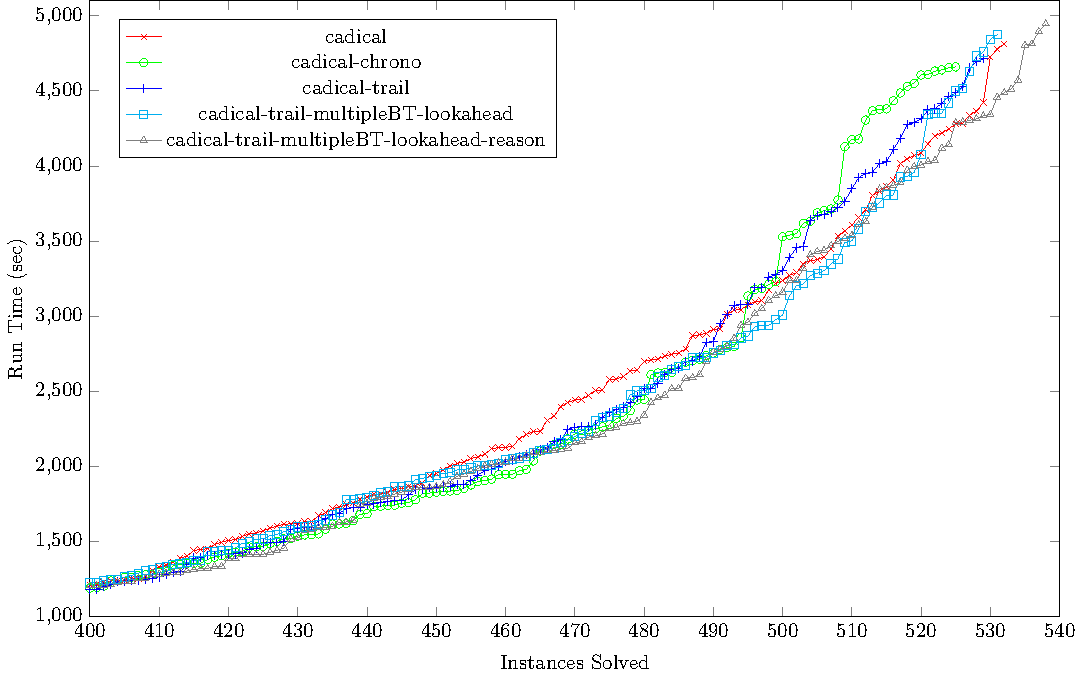
\includegraphics[scale=0.65]{figures/cactus_cadical_new.pdf}\caption{\small{Cactus plot for the newest version of cadical comparing standard non-chronological backtracking to \cbt and various configurations of trail saving. The first 400 problems were solved in less than 1200 seconds, so that part of the plot is truncated.}}\label{fig:cactus_cadical}\end{figure}

\begin{figure}\centering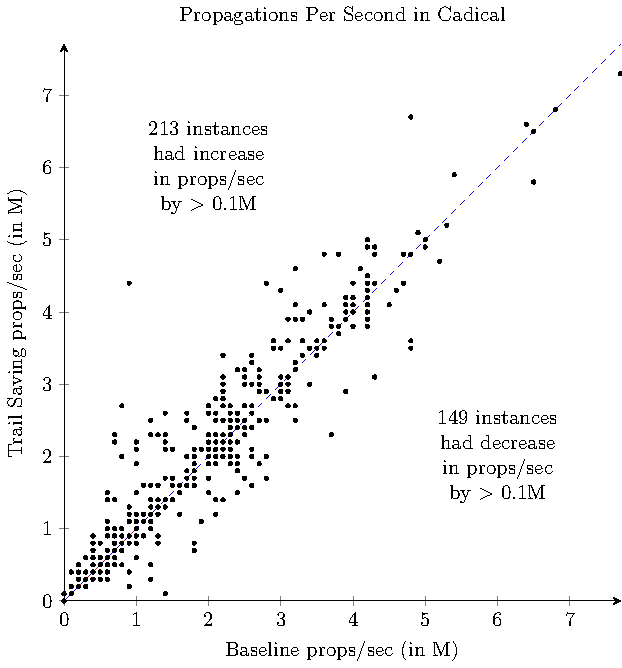
\includegraphics[scale=0.7]{figures/scatter.pdf}\caption{Comparing propagations per second with and without trail saving in Cadical.}\label{fig:props}\end{figure}

\section{Conclusion}
We have shown that our method trail saving can speed up two
state-of-the-art \sat solvers, cadical and MapleSAT, about as well as
chronological backtracking can without breaking the conventional invariants
of CDCL. We also introduced three enhancements one can
implement when using a saved trail and demonstrated experimentally
that these enhancements can sometimes improve a solver's performance by a significant
amount. We have shown that trail saving and all enhancements we proposed are sound.
A line of future work might include introducing further enhancements,
such as using the saved trail to help make inprocessing techniques faster or
using the saved trail to learn a second learnt clause from a single conflict.
It is also possible to combine trail saving with chronological
backtracking if one is willing to break the traditional invariants of CDCL,
but we leave it to future work to determine whether or not this would be
useful and how to best approach it.


%\section{Future Work}

%With more clever data structures the efficiency of restoring the trail
%could be improved. There are a number of parameters which can be
%tuned, including how often to refresh the trail, how large the cutoff
%point for rejecting "long" reasons should be, how long to wait to
%prune the trail cache if one is appending multiple trail caches
%together, how far to look ahead on the trail cache for conflicts (in
%terms of number of decisions or total number of literals). We only
%experimented with a few different settings of these parameters that
%made sense, but more careful fine-tuning of these parameters could
%further enhance the effectiveness of the technique. There are
%potentially other techniques one could use a trail cache for,
%including inprocessing steps that involve probing. A look down the
%trail cache is an incomplete but very fast way to do a probing step,
%as opposed to propagation. It is also possible that trail saving and
%chronological backtracking could be combined in some way to produce
%even better results.

\bibliography{sat}{}
\bibliographystyle{splncs04}
\end{document}

\iffalse \textit{Example 1} Suppose the literal $y$ can be restored
from the trail cache, and its reason clause $cr$ contains the literals
${y \lnot x_1, \lnot x_2, ..., \lnot x_n}$. This means that
$x1, ..., x_n$ have become true and are currently on the
trail. Suppose $x_n$ is the most recent literal on the trail and
Without trail saving, the propagation routine will have to access $cr$
from the watchlist of one of the literals $\blacksquare$\newline

\textit{Example 1} Suppose the literals $x_1, ... x_n$ are on the
trail cache, with none of them having a null reason, and $x_1$ becomes
true (e.g., the solver makes a decision for $x_1$ to be true). Then,
$x_2, ... x_n$ are implied by the current trail. Now we will examine
the propagation of a clause c which consists of the literals
$l, \lnot x_1, \lnot x_2, ..., \lnot x_n$ with and without trail
saving. Assume $l$ and $\lnot x_1$ are the current watched literals.

Without trail saving, $\lnot x_1$ becomes false and a new watcher is
searched for and found 1 literal later, $\lnot x_2$, and then
$\lnot x_1$ and $\lnot x_2$ are swapped. Next $\lnot x_2$ becomes
false, a new watcher is searched for and found 2 literals later,
$\lnot x_3$, and then $\lnot x_2$ and $\lnot x_3$ are swapped. This
process will continue until all $x_n$ literals are false, c becomes
unit, and $l$ becomes forced to be true. This propagation took
$1 + 2 + ... + n$ searches through clause c, for a total of $O(n^2)$
searches.

With trail saving, $x2, ... x_n$ are all assigned to be true as soon
as $x_1$ is made true, so immediately the values of literals
$\lnot x_1, ..., \lnot x_n$ in c are false. During propagation, a new
watcher is searched for to replace $\lnot x_2$, n literals are
searched over without finding any, thus c is detected as unit and $l$
becomes forced to be true. This propagation took $O(n)$ searches
through clause c. $\blacksquare$\newline \fi

\iffalse
\begin{figure}\includegraphics[scale=0.8]{figures/cactus_cadical.pdf}\caption{\small{Comparison
        of run times for versions of cadical. cadical is without
        chronological backtracking, cadical-chrono is with
        chronological backtracking, cadical-trail is with the first
        version of trail saving, cadical-trail-2levels-ahead is the
        trail saving with all enhancements added.}}\end{figure}
\begin{figure}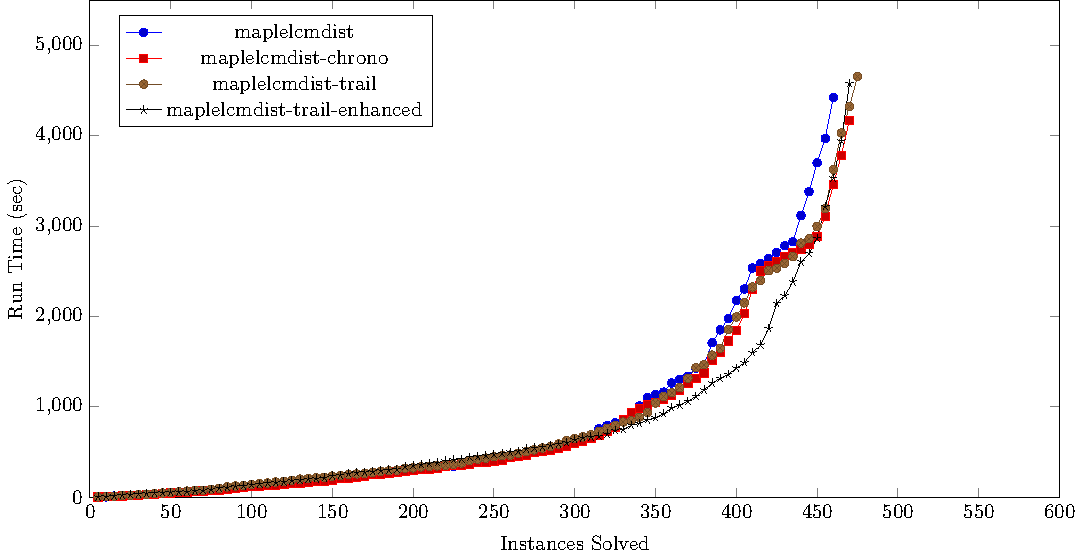
\includegraphics[scale=0.8]{figures/cactus_maple2.pdf}\caption{\small{Comparison
        of run times for versions of MapleSAT. maplelcmdist is from
        the 2017 SAT Competition, maplelecmdist-chrono is with
        chronological backtracking (2018 SAT Competition),
        maplelcmdist-trail is with the first version of trail saving,
        maplelcmdist-trail-enhanced is with trail saving and all
        enhancements added.}}\end{figure}
\begin{figure}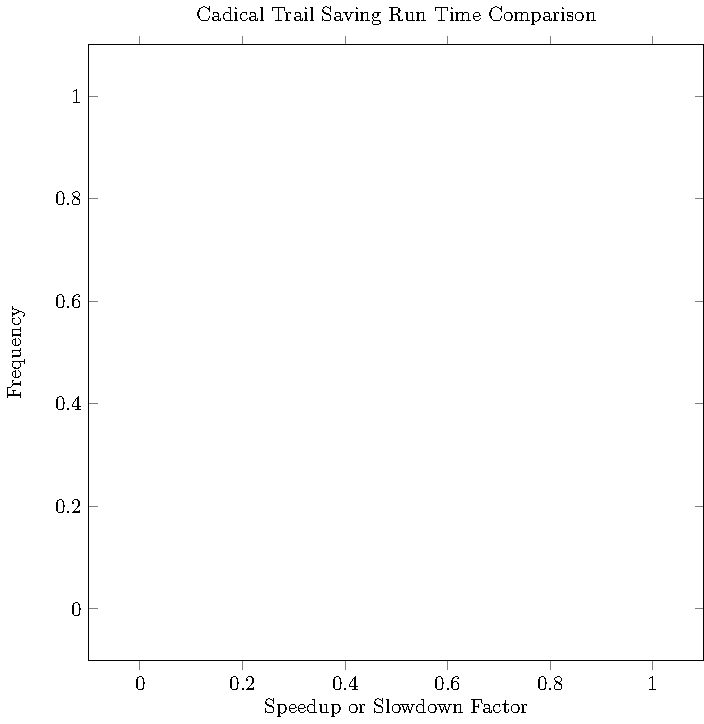
\includegraphics[scale=0.8]{figures/test.pdf}\caption{}\end{figure}
\begin{figure}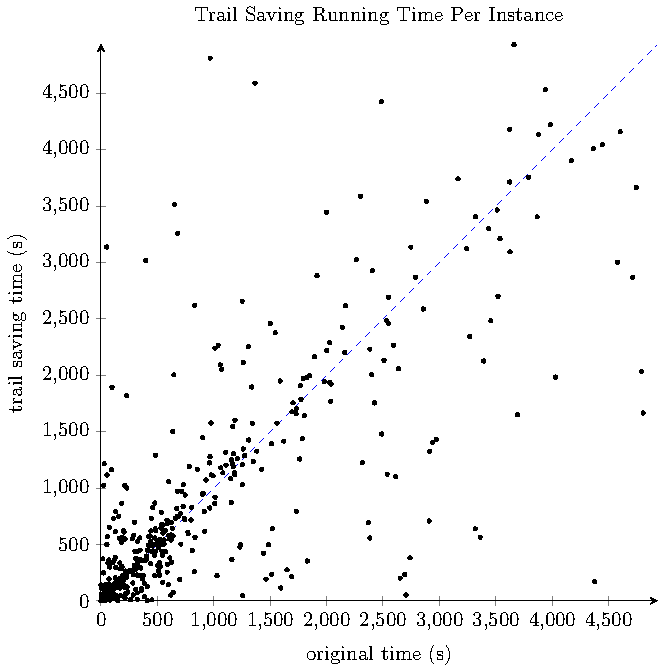
\includegraphics[scale=0.8]{figures/test2.pdf}\caption{}\end{figure}
\fi
\iffalse
\begin{figure}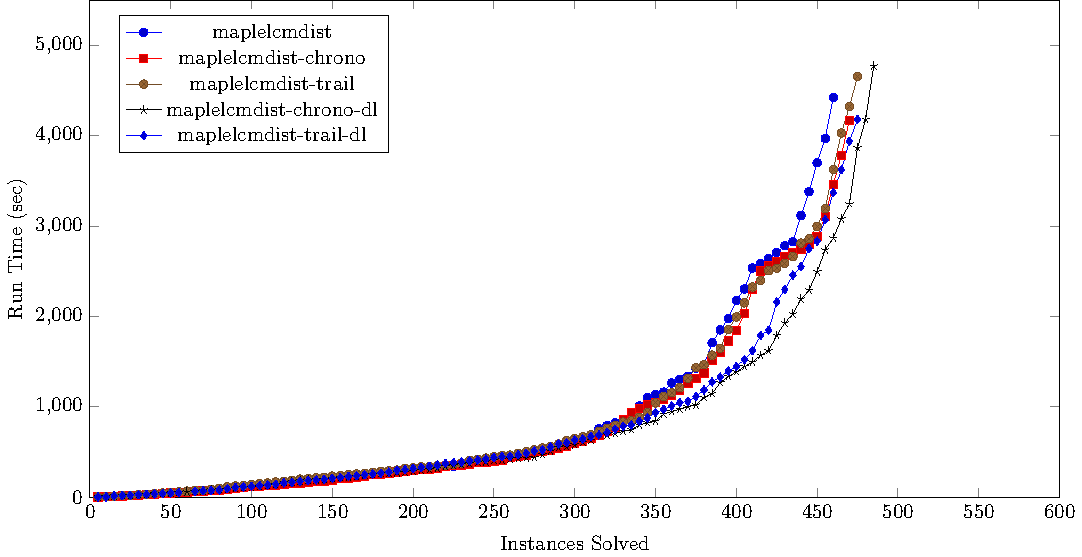
\includegraphics[scale=0.8]{figures/cactus_maple.pdf}\caption{\small{Comparison
        of run times for versions of MapleSAT. maplelcmdist is from
        the 2017 SAT Competition, maplelecmdist-chrono is with
        chronological backtracking (2018 SAT Competition),
        maplelcmdist-trail is with the first version of trail saving,
        maplelcmdist-chrono-dl is with chronological backtracking and
        duplicate learnts (2019 SAT Competition),
        maplelcmdist-trail-dl is with trail saving and duplicate
        learnts}}\end{figure}
\fi

\iffalse
\begin{figure}[t]
    \begin{center}
        \fss{9pt}{10pt}
        \setlength\tabcolsep{1pt}
        \begin{tabular}{| p{4.2cm} | c | c | c | c | c | c | c | c |}
          \hline
          & \multicolumn{4}{|c|}{Total} & \multicolumn{2}{|c|}{Unweighted} & \multicolumn{2}{|c|}{Weighted} \\ \hline
          & MaxHS & +/- & \hspace{1pt} RC2 \hspace{1pt} & +/- & MaxHS & \hspace{1pt} RC2 \hspace{1pt} & MaxHS & \hspace{1pt} RC2 \hspace{1pt} \\ \hline
          original & 6052 & 0/0 & 6030 & 0/0 & 3940 & 3993 & 2112 & 2037 \\ \hline
          enqueue assumptions as set & 6131 & 114/35 & 6081 & \hspace{0.5pt} 99/48 \hspace{0.5pt} & 3995 & 4032 & 2136 & 2049 \\ \hline
          enqueue assumptions as set + \newline save literals after learnt units & 6136 & 120/36 & 6079 & \hspace{0.5pt} 95/46 \hspace{0.5pt} & 3991 & 4030 & 2145 & 2049 \\ \hline
          enqueue assumptions as set + \newline save literals after learnt units + \newline save literals from last invocation & 6138 & 115/29 & 6080 & \hspace{0.5pt} 92/42 \hspace{0.5pt} & 3989 & 4030 & 2149 & 2050 \\ \hline
        \end{tabular}
    \end{center}
    \caption{Number of \maxsat instances solved by MaxHS and RC2 using
      different extensions of the underlying \sat solver. The +/- column shows
      the number of instances gained/lost vs the original.}
    \label{fig:nsolved}
\end{figure}
\fi
